\documentclass[11pt]{article}
\usepackage{epstopdf}
\usepackage{amssymb,amsmath}
%\usepackage{subfigure}
\usepackage{subcaption}
\usepackage{graphicx}
\usepackage[]{algorithm2e}
\usepackage{xcolor,listings}
\usepackage{multirow}
\title{Report for CS739 Key-value Store Project}
\author{Ce Zhang, Shu Wang, Jing Fan\\
        Partner Group: Menghui Wang, Lichao Yin, Shike Mei}

\begin{document}
\maketitle
\section{Implementation}
\begin{figure}[htp]
\caption{Client And Server}
\label{fig:clientandserver} \centering{
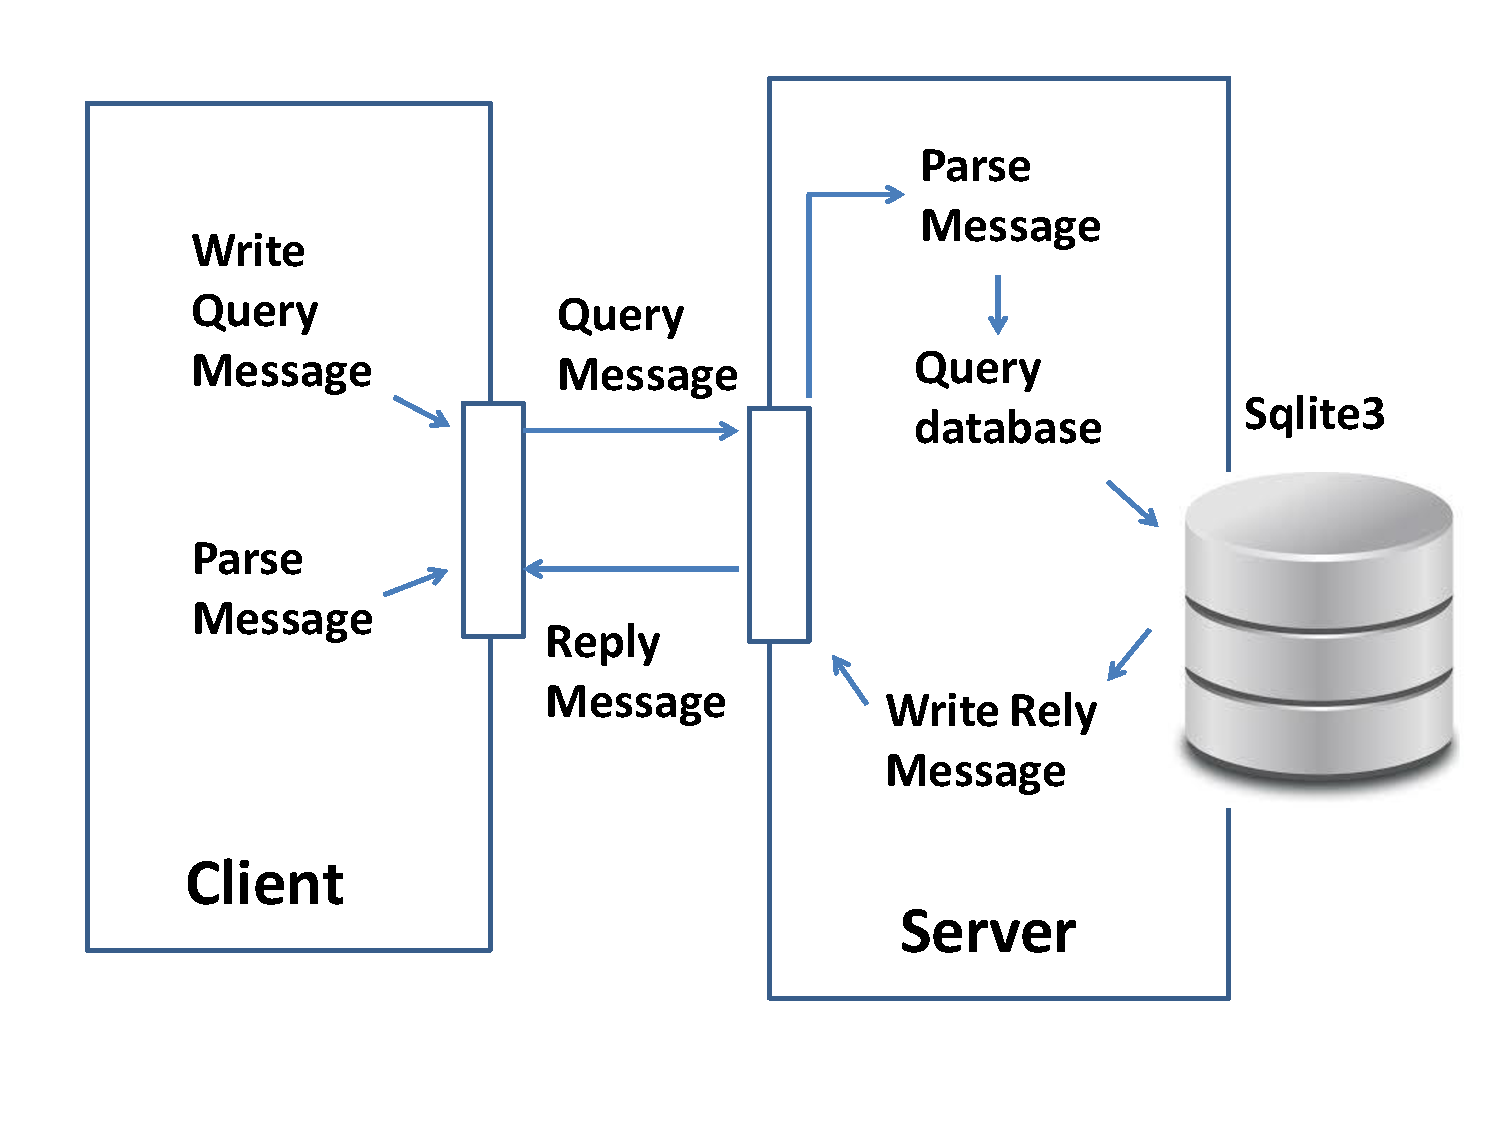
\includegraphics[scale=0.4]{client_server.pdf}}
\end{figure}
 We illustrate the implementation of client and server in Figure~\ref{fig:clientandserver}. 
 \subsection{Communication}
 Client and server uses TCP socket to do network communication. Server will bind to a socket when it starts. We also implemented a flexible message wrapper for client and server to serialize and deserialize the message.
 \subsection{Storage}
 Server uses SQLite3 as backend data storage engine and the key-value pairs will be stored in the table \textsf{kvstore} in the database \textsf{739.db}. When the server starts, it will first create/connect to the databse \textsf{739.db}. If the table \textsf{kvstore} already exist, the server will finish initialization and listen to the clients' requests. Otherwise, the table \textsf{kvstore} will be created according to the SQL in Listing\ref{listing:createkvstore}. In SQLite3, the data is persistent and the server can achieve fault tolerance.
\begin{lstlisting}[
           language=SQL,
           caption={Create the Table kvstore},
           label={listing:createkvstore},
        ]
CREATE TABLE kvstore(
key char[129],
value char[2049]
);
\end{lstlisting}
 \subsection{Init}
 The client will connect to server according to the ip address and port number given by the user.
 \subsection{Get}
 The client specifies the key to retrieve value and send a query message to the server. The server will parse the message and query the database using the key. After getting the query result, the server will write a reply message to the client.
 \subsection{Put}
The server will first query the result will the key given, if there is such key in database, the server will update the database by setting the new value. Otherwise, it will insert the new key-value pair into database. Then a reply message is written and sent.
\section{Communication Protocol}
 \begin{table}
    \caption{Query Message}
    \begin{tabular}{|c|c|c|}
    \hline
    \textbf{Type} &  \multicolumn{2}{| c |}{\textbf{String(Several)} }\\
    \hline
    Operation Type(int, 4 bytes) & String length(int, 4 bytes) & String(char array)\\
    \hline
    \end{tabular}
 \end{table}
 
 \begin{table}
    \caption{Reply Message}
    \begin{tabular}{|c|c|c|}
    \hline
    \textbf{Return Value} &  \multicolumn{2}{| c |}{\textbf{String(If any)} }\\
    \hline
    Return value(int, 4 bytes) & String length(int, 4 bytes) & String(char array)\\
    \hline
    \end{tabular}
 \end{table}
 Query Message: The first 4 bytes indicate the operation type, 0 for get operation and 1 for put operation. A string is expressed in combination of a 4 bytes int value and a char array. The 4 bytes int indicates the length of the char array. The message can contain one string(key) or two strings(key and value in put operation).
 Reply Message: The first 4 bytes indicate the return value. The message may contain 0 string or 1 string(old$\_$value in put operation).
 
\end{document}
